\documentclass[11pt]{article}

% Load packages
\usepackage{float} % for formatting figures
\usepackage{amsmath, amsfonts, breqn} % for math
\usepackage{graphicx} % for figures
\usepackage[margin=1in]{geometry} % to set margins
\usepackage{tcolorbox} % to create nice boxes
\tcbuselibrary{skins,breakable} % extra libraries for the nice boxes

% Define a custom box for the solutions. Don't change this!
\newtcolorbox[]{solution}
    {colframe=red!20, 
        colback=white, 
        sharp corners,
        title=Solution,
        enhanced,
        coltitle=black,
        fonttitle=\bfseries,
        attach boxed title to top left={yshift*=-\tcboxedtitleheight/2, xshift=3mm},
        boxed title style={sharp corners, colback=red!20}
        }

\usepackage{hyperref}
\hypersetup{
    colorlinks=true,
    linkcolor=blue,
    filecolor=magenta,      
    urlcolor=cyan
}



% Write the document
\begin{document}

  \section{Problem 1:  Couette Flow}
    Couette flow is a classic basic flow pattern in which a fluid is confined between two, smooth parallel plates.  The
bottom plate (at $y=-h$) is stationary while the top plate (at $y=h$) is moving with a constant velocity $U$.  It is assumed
that the flow is:
    \begin{enumerate}
      \item Steady
      \item Fully developed
      \item Two-dimensional (independent of $z$)
      \item Zero pressure-gradient
    \end{enumerate}
    Use no-slip boundary conditions.  Figure~\ref{fig:couette} shows a diagram of the flow configuration.
    \begin{figure}[h!]
      \centering
      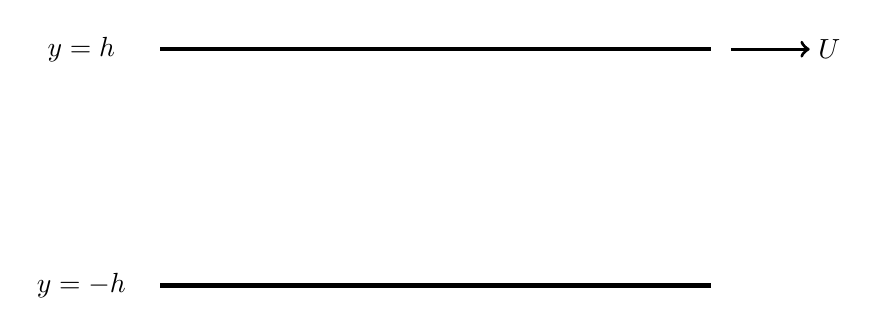
\begin{tikzpicture}
        \draw [ultra thick] (3,0) -- (10,0);
        \draw [ultra thick] (3,-3) -- (10,-3);
        \draw [very thick, ->] (10.25,0) -- (11.25,0);
        \node at (2.0, 0) [] {$y=h$};
        \node at (2.0, -3) [] {$y=-h$};
        \node at (11.5, 0) [] {$U$};
      \end{tikzpicture}
      \caption{The Couette flow configuration.}
      \label{fig:couette}
    \end{figure}

    \textbf{Calculate the following:}
    \begin{enumerate}
      \item The velocity field 
      \item The vorticity field
      \item The shear stress
      \item The volume flow rate 
      \item The average and maximum velocities in the channel
        \begin{itemize}
          \item Hint:  $u_{\textrm{ave}} = Q / h$ where $Q$ is the volume flow rate.
        \end{itemize}
    \end{enumerate}

    \textbf{Plot:}
    Make a plot of the velocity profile at a few different values of $U$.  Put $y$ on the $y-$ axis and $u\left(y\right)$ on
the $x-$ axis.

\graphicspath{ {./YX/} }

\begin{solution}

  \subsection{Mathematical Formulation}
    The Couette Flow obeys the following equations of motion:
    \begin{align}
      \nabla\cdot\mathbf{u}&=0 \label{eq:continuity}\\
      \rho\left(\frac{\partial\mathbf{u}}{\partial t}+\mathbf{u}\cdot\nabla\mathbf{u}\right)
      &=-\nabla P+\mu\nabla^2\mathbf{u} \label{eq:momentum}
    \end{align}
    Eq.(\ref{eq:continuity}) is known as the equation of continuity, and Eq.(\ref{eq:momentum}) describes the conservation of momentum. Other assumptions in this problem are translated as follows:
    \begin{enumerate}
      \item Steady
        \begin{equation}
          \frac{\partial (\cdot)}{\partial t}=0
        \end{equation}
      \item Fully developed
        \begin{equation}
          \frac{\partial\mathbf{u}}{\partial x}=0
        \end{equation}
      \item Two-dimensional
        \begin{equation}
          \frac{\partial (\cdot)}{\partial z}=0
        \end{equation}
      \item Zero pressure-gradient
        \begin{equation}
          \nabla P=0
        \end{equation}
      \item No-slip boundary
        \begin{equation}
          \mathbf{u}\big|_{y=-h}=0, \quad
          \mathbf{u}\big|_{y=h}=U\hat{\mathbf e}_x
        \end{equation}
    \end{enumerate}
    Putting them all together, we have the well-posed problem for $\mathbf{u}=u(y)\hat{\mathbf{e}}_x+v(y)\hat{\mathbf{e}}_y$:
    \begin{align}
      \frac{\partial v}{\partial y}&=0 \\
      v\frac{\partial u}{\partial y}&=\frac{\mu}{\rho}\frac{\partial^2 u}{\partial y^2} \\
      v\big|_{y=-h}=0&,\quad v\big|_{y=h}=0 \\
      u\big|_{y=-h}=0&,\quad u\big|_{y=h}=U
    \end{align}

\end{solution}



\begin{solution}
    
  \subsection{The Velocity Field}
    We first note that $v$ has its own independent boundary problem, \emph{i.e.}
    \begin{align}
      \frac{\partial v}{\partial y}&=0 \\
      v\big|_{y=-h}=0&,\quad v\big|_{y=h}=0
    \end{align}
    whose solution is:
    \begin{align}
      v=0
    \end{align}
    Plugging it back, we rewrite the problem for $u$:
    \begin{align}
      \frac{\partial^2 u}{\partial y^2}&=0 \\
      u\big|_{y=-h}=0&,\quad u\big|_{y=h}=U
    \end{align}
    So the solution for $u$ is:
    \begin{align}
      u=\frac{U}{2}\left(1+\frac{y}{h}\right)
    \end{align}
    Putting them together we have the full solution for the velocity field:
    \begin{align}
      \mathbf{u}=\frac{U}{2}\left(1+\frac{y}{h}\right)\hat{\mathbf{e}}_x
    \end{align}
    \begin{figure}[H]
      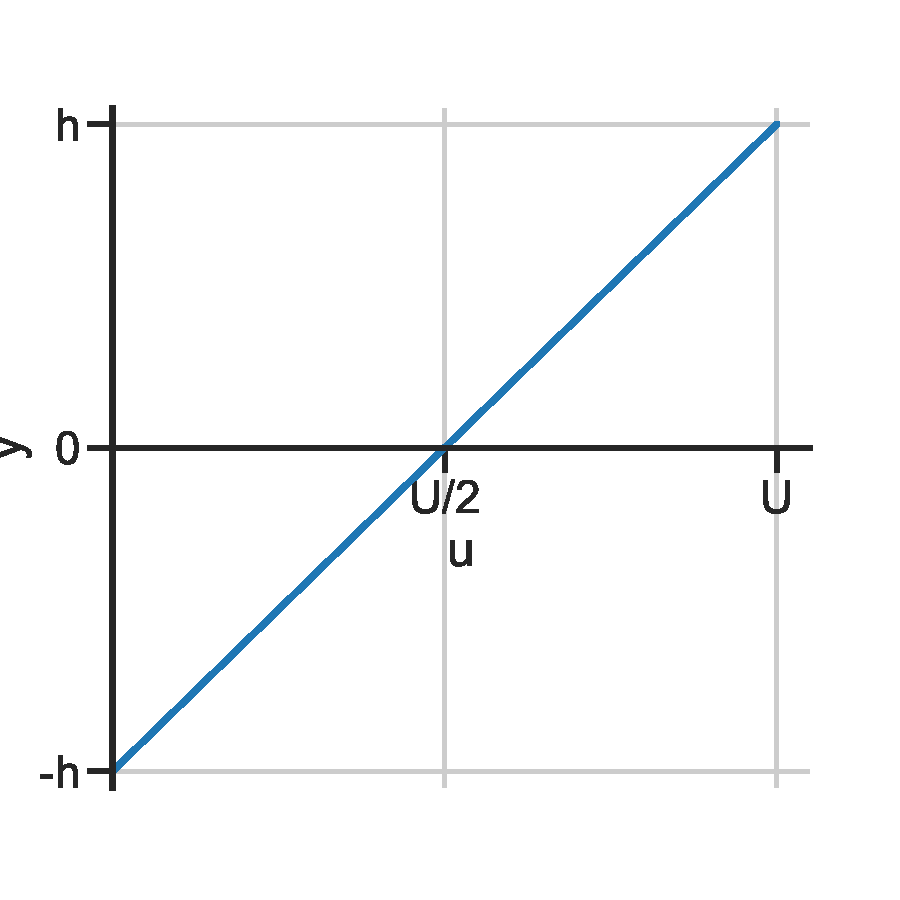
\includegraphics[scale=0.5]{YX/velocity_profile.pdf}
      \centering
      \caption{Velocity Profile}
    \end{figure}
    
\end{solution}



\begin{solution}

  \subsection{The Vorticity Field}
    \begin{align}
      \omega=\nabla\times\mathbf{u}=-\frac{U}{2h}\hat{\mathbf{e}}_z
    \end{align}
    
  \subsection{The Shear Stress}
    \begin{align}
      \tau=\mu\left(\nabla\mathbf{u}+\nabla\mathbf{u}^T\right)=\frac{\mu U}{2h}\left(\hat{\mathbf{e}}_{xy}+\hat{\mathbf{e}}_{yx}\right)
    \end{align}
  
  \subsection{The Volume Flow Rate}
    \begin{align}
      Q=\int_{-h}^{h}\!u~\text{d}y=Uh
    \end{align}

  \subsection{The Average and Maximum Velocity}
    \begin{align}
      u_{ave}&=\frac{Q}{2h}=\frac{U}{2} \\
      u_{max}&=U
    \end{align}
    

\end{solution}

\newpage
    \section{Problem 2:  Rectangular Duct Flow}
    Consider flow through a duct of rectangular cross section as shown in Figure~\ref{fig:rect_duct}.  Make the following
assumptions:
    \begin{itemize}
      \item $1$-component flow (that is $v = w = 0$)
      \item Fully developed flow in $x$
      \item Steady flow
    \end{itemize}
    Use no-slip boundary conditions on all surfaces.  Finally, note that the flow is driven by a prescribed (known) pressure
gradient in the $x-$ direction.

    \begin{figure}[h!]
      \centering
      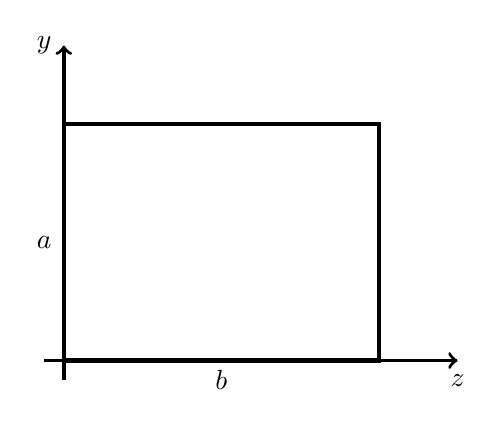
\begin{tikzpicture}
        \draw [ultra thick] (0,0) rectangle (4,3);
        \draw [very thick, ->] (0,-0.25) -- (0,4);
        \draw [very thick, ->] (-0.25,0) -- (5,0);
        \node at (5, -0.25) {$z$};
        \node at (-0.25, 4) {$y$};
        \node at (2, -0.25) {$b$};
        \node at (-0.25, 1.5) {$a$};
      \end{tikzpicture}
      ~~~
      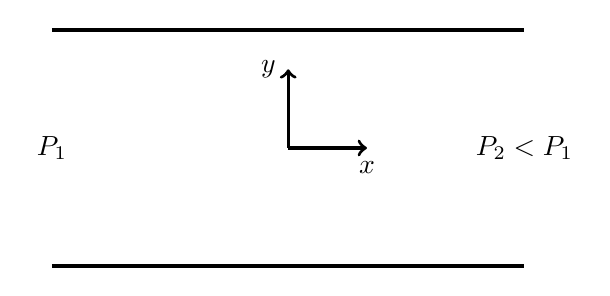
\begin{tikzpicture}
        \draw [ultra thick] (0,3) -- (6,3);
        \draw [ultra thick] (0,0) -- (6,0);
        \draw [very thick, ->] (3,1.5) -- (4,1.5);
        \draw [very thick, ->] (3,1.5) -- (3,2.5);
        \node at (4, 1.25) {$x$};
        \node at (2.75, 2.5) {$y$};
        \node at (0, 1.5) {$P_{1}$};
        \node at (6, 1.5) {$P_{2} < P_{1}$};
      \end{tikzpicture}
      \caption{Left:  Cross-section of the rectangular duct. Right: Profile of rectangular duct.}
      \label{fig:rect_duct}
    \end{figure}

    \subsection{Governing Equations}
    Using the provided assumpsions, show that the Navier-Stokes equations reduce to, 
    \begin{align}
      \partial_{y}^{2}u + \partial_{z}^{2}u = \frac{1}{\mu}\partial_{x}P.
    \end{align}
    \textbf{What are the boundary conditions?}

\begin{solution} 

Because $v = w = 0$, we can only consider the momentum equation for the $u$ component:
    \begin{align*}
      \rho(\partial_{t}u + u\partial_{x}u + v\partial_{y}u + w\partial_{z}u) = - \partial_{x}P + {\mu}(\partial_{x}^{2}u + \partial_{y}^{2}u + \partial_{z}^{2}u)
    \end{align*}

    \begin{itemize}
    	\item $v\partial_{y}u + w\partial_{z}u$ can be removed because $v = w = 0$
	\item ``Fully developed in $x$" means $\partial_{x}u=0$, thus the $u\partial_{x}u$ and $\partial_{x}^{2}u$ terms above can be removed. Steady flow means 
   	\item ``Steady flow" means  $\partial_{t}u=0$
    \end{itemize}
   
The remaining terms are:
       \begin{align*}
      0 = - \partial_{x}P + {\mu}(\partial_{y}^{2}u + \partial_{z}^{2}u)
    \end{align*}

Re-arranging them leads to:
    \begin{align*}
      \partial_{y}^{2}u + \partial_{z}^{2}u = \frac{1}{\mu}\partial_{x}P
    \end{align*}
    
The no-slip boundary conditions are 
    \begin{align*}
      u(y=0) = u(y=a) = u(z=0) = u(z=b) = 0
    \end{align*}

\end{solution} 

    \subsection{Solving for $u$: Part 1}
    We have an inhomogenous, linear PDE on our hands.  Let's solve this using the method of eigenfunction expansions.  We
know that with the current boundary conditions, the homogenous solution to our equation has eigenfunctions that are sines.
Hence, let's assume a solution of the form,
    \begin{align}
      u\left(y, z\right) = \sum_{n=1}^{\infty}{\beta_{n}\left(z\right)\sin\left(\frac{n\pi}{a}y\right)}.
    \end{align}
    Plug this assumed form into the governing PDE and show that the unknown coefficients ($\beta_{n}\left(z\right)$) are
governed by the following inhomogenous ODE,
    \begin{align}
      \beta_{n}^{\prime\prime} - \gamma_{n}^{2}\beta_{n} = q_{n} \label{eq:betan}
    \end{align}
    where $\left(\cdot\right)^{\prime}$ denotes $d/dz$, 
    \begin{align}
      \gamma_{n} = \frac{n\pi}{a}
    \end{align}
    and 
    \begin{align}
      q_{n} = \dfrac{2}{a}\int_{0}^{a}{Q\sin\left(\gamma_{n}y\right)\ \mathrm{d}y}, \qquad Q = \frac{1}{\mu}\partial_{x}P.
    \end{align}

    \subsubsection{Some Specific Details}
    Here is a breakdown of the required steps.
    \begin{enumerate}
      \item First show that after plugging the assumed form into the governing PDE the
resulting expression is 
      \begin{align}
        \sum_{n=1}^{\infty}{\beta_{n}^{\prime\prime}\sin\left(\dfrac{n\pi}{a}y\right)} -
\sum_{n=1}^{\infty}{\beta_{n}\left(\dfrac{n\pi}{a}\right)^{2}\sin\left(\dfrac{n\pi}{a}y\right)} = Q.
      \end{align}
      \item Next, multiply by $\sin\left(\dfrac{m\pi}{a}y\right)$ and integrate over $y$.
      \begin{align}
        &\int_{0}^{a}{\sum_{n=1}^{\infty}{\beta_{n}^{\prime\prime}\sin\left(\dfrac{n\pi}{a}y\right)\sin\left(\dfrac{m\pi}{a}y\right)}
\ \mathrm{d}y} -
\int_{0}^{a}{\sum_{n=1}^{\infty}{\beta_{n}\left(\dfrac{n\pi}{a}\right)^{2}\sin\left(\dfrac{n\pi}{a}y\right)\sin\left(\dfrac{m\pi}{a}y\right)}
\ \mathrm{d}y} = \nonumber \\
        &\hspace{2.0em}\int_{0}^{a}{Q\sin\left(\dfrac{m\pi}{a}y\right) \ \mathrm{d}y}.
      \end{align}
      \item That's a pretty big mess.  Now, we use a beautiful result:  the orthogonality of sines:
        \begin{align}
          \int_{0}^{a}{\sin\left(\dfrac{n\pi}{a}y\right)\sin\left(\dfrac{m\pi}{a}y\right) \ \mathrm{d}y} = 
          \left\{
            \begin{array}{ll}
              0            \qquad n \neq m \\
              \dfrac{a}{2} \qquad n = m
            \end{array}
          \right.
        \end{align}
        The main point here is that every single term in the infinite sum is zero \textit{except} for the term where $n=m$.
      \item The final result is 
        \begin{align}
          \beta_{n}^{\prime\prime} - \gamma_{n}^{2}\beta_{n} = \dfrac{2}{a}\int_{0}^{a}{Q\sin\left(\gamma_{n}y\right) \ \mathrm{d}y}
        \end{align}
    \end{enumerate}

    \textbf{What are the boundary conditions on $\beta_{n}$}?

\begin{solution} 

Start with
    \begin{align*}
      u\left(y, z\right) = \sum_{n=1}^{\infty}{\beta_{n}\left(z\right)\sin\left(\frac{n\pi}{a}y\right)}.
    \end{align*}

Take second-order derivatives:
    \begin{align*}
      \partial_{y}^{2}u &= - \sum_{n=1}^{\infty} (\frac{n\pi}{a})^2 {\beta_{n} \left(z\right)\sin\left(\frac{n\pi}{a}y\right)} \\
      \partial_{z}^{2}u &= \sum_{n=1}^{\infty}{\beta_{n}^{\prime\prime} \left(z\right)\sin\left(\frac{n\pi}{a}y\right)}
    \end{align*}

Bring into the original PDE:
    \begin{align*}
      \partial_{y}^{2}u + \partial_{z}^{2}u = Q
    \end{align*}

Leads to:
      \begin{align*}
        \sum_{n=1}^{\infty}{\beta_{n}^{\prime\prime}\sin\left(\dfrac{n\pi}{a}y\right)} -
\sum_{n=1}^{\infty}{\beta_{n}\left(\dfrac{n\pi}{a}\right)^{2}\sin\left(\dfrac{n\pi}{a}y\right)} = Q
      \end{align*}

Multiply by $\sin\left(\dfrac{m\pi}{a}y\right)$ and integrate over $y$:
      \begin{align*}
        &\int_{0}^{a}{\sum_{n=1}^{\infty}{\beta_{n}^{\prime\prime}\sin\left(\dfrac{n\pi}{a}y\right)\sin\left(\dfrac{m\pi}{a}y\right)}
\ \mathrm{d}y} -
\int_{0}^{a}{\sum_{n=1}^{\infty}{\beta_{n}\left(\dfrac{n\pi}{a}\right)^{2}\sin\left(\dfrac{n\pi}{a}y\right)\sin\left(\dfrac{m\pi}{a}y\right)}
\ \mathrm{d}y} = \nonumber \\
        &\hspace{2.0em}\int_{0}^{a}{Q\sin\left(\dfrac{m\pi}{a}y\right) \ \mathrm{d}y}
      \end{align*}

Using the orthogonality of sines, it becomes:
        \begin{align*}
           \dfrac{a}{2}\beta_{m}^{\prime\prime} - \dfrac{a}{2}(\dfrac{m\pi}{a})^{2}\beta_{m} =\int_{0}^{a}{Q\sin\left(\dfrac{m\pi}{a}y\right) \ \mathrm{d}y}
        \end{align*}

Replace $m$ by $n$ (they are interchangeable at the above step) and use $\gamma_{n}=\dfrac{n\pi}{a}$, the above reduces to the desired result:
        \begin{align*}
          \beta_{n}^{\prime\prime} - \gamma_{n}^{2}\beta_{n} = \dfrac{2}{a}\int_{0}^{a}{Q\sin\left(\gamma_{n}y\right) \ \mathrm{d}y}
        \end{align*}

\end{solution} 

    \subsection{Solving for $\beta_{n}$: The Homogeneous Part}
    To solve for $\beta_{n}$, we first need to solve the homogeneous equation,
    \begin{align}
      \beta_{n}^{\prime\prime} - \gamma_{n}^{2}\beta_{n} = 0.
    \end{align}
    Show that the homogeneous solution is 
    \begin{align}
      \beta_{n}^{H} = c_{1}w_{1} + c_{2}w_{2}
    \end{align}
    where $w_{1} = \sinh\left(\gamma_{n}z\right)$ and $w_{2} = \cosh\left(\gamma_{n}z\right)$ are the two linearly
independent solutions.

\begin{solution} 

The homogeneous ODE can be factored (in terms of operators) as:
    \begin{align*}
    (\dfrac{d}{dz}-\gamma_{n}) (\dfrac{d}{dz}+\gamma_{n})\beta_{n}= 0
    \end{align*}

The solution needs to satisfy either:
    \begin{align*}
    (\dfrac{d}{dz}-\gamma_{n})\beta_{n} = 0 \text{  or  } (\dfrac{d}{dz}+\gamma_{n})\beta_{n} = 0
    \end{align*}
    
The solution to each first-order ODE is:
    \begin{align*}
    \beta_{n} = e^{\gamma_{n}z} \text{  or  } \beta_{n} = e^{-\gamma_{n}z}
    \end{align*}

Any of their linear combinations are correct solutions:
    \begin{align*}
    \beta_{n}^{H} = k_1 e^{\gamma_{n}z} + k_2 e^{-\gamma_{n}z}
    \end{align*}

Or, equivalently
    \begin{align*}
      \beta_{n}^{H} = c_{1} \sinh\left(\gamma_{n}z\right) + c_{2} \cosh\left(\gamma_{n}z\right)
    \end{align*}

\end{solution} 

    \subsection{Solving the Inhomogeneous Part}
    You can use the method of variation of parameters to solve the inhomogeneous equation.  Let 
    \begin{align}
      \beta_{n}\left(z\right) = v_{1}\left(z\right)w_{1}\left(z\right) + v_{2}\left(z\right)w_{2}\left(z\right)
      \label{eq:var_param}
    \end{align}
    where $v_{1}\left(z\right)$ and $v_{2}\left(z\right)$ are the coefficients (parameters) to be varied.  Now
\textit{assume} that 
    \begin{align}
      w_{1}v_{1}^{\prime} + w_{2}v_{2}^{\prime} = 0. \label{eq:var_const}
    \end{align}
    Then, by plugging~\eqref{eq:var_param} into~\eqref{eq:betan} and using~\eqref{eq:var_const} yields two equations for
$v_{1}^{\prime}$ and $v_{2}^{\prime}$.  These two equations are, 
    \begin{align}
      w_{1}v_{1}^{\prime} + w_{2}v_{2}^{\prime} &= 0 \\
      w_{1}^{\prime}v_{1}^{\prime} + w_{2}^{\prime}v_{2}^{\prime} &= q_{n}.
    \end{align}
    Show that 
    \begin{align}
      v_{1} &= \frac{q_{n}}{\gamma_{n}^{2}}\sinh\left(\gamma_{n}z\right) + \alpha_{1} \\
      v_{2} &= -\frac{q_{n}}{\gamma_{n}^{2}}\cosh\left(\gamma_{n}z\right) + \alpha_{2} 
    \end{align}
    where $\alpha_{1}$ and $\alpha_{2}$ are constants of integration.

    Finally, show that 
    \begin{align}
      \beta_{n}\left(z\right) &= C_{n} 
        \left[-\sinh\left(\gamma_{n}b\right) + \sinh\left(\gamma_{n}z\right) - 
          \left(\sinh\left(\gamma_{n}z\right)\cosh\left(\gamma_{n}b\right) - 
            \cosh\left(\gamma_{n}z\right)\sinh\left(\gamma_{n}b\right)\right)\right] \\
      &=  C_{n}
           \left[\sinh\left(\gamma_{n}z\right) - \sinh\left(\gamma_{n}b\right) - 
            \sinh\left(\gamma_{n}\left(z-b\right)\right)\right] \\
      &= 2C_{n}\sinh\left(\dfrac{\gamma_{n}}{2}\left(z-b\right)\right) 
           \left[\cosh\left(\dfrac{\gamma_{n}}{2}\left(z+b\right)\right) - 
             \cosh\left(\dfrac{\gamma_{n}}{2}\left(z-b\right)\right)\right].
    \end{align}
    where 
    \begin{align}
      C_{n} = \frac{q_{n}}{\gamma_{n}^{2}\sinh\left(\gamma_{n}b\right)}. 
    \end{align}

\begin{solution} 

Start with 
    \begin{align*}
      w_{1}v_{1}^{\prime} + w_{2}v_{2}^{\prime} &= 0 \\
      w_{1}^{\prime}v_{1}^{\prime} + w_{2}^{\prime}v_{2}^{\prime} &= q_{n}
    \end{align*}

Or equivalently,
    \begin{align*}
      \sinh({\gamma_{n}z}) v_{1}^{\prime} + \cosh({\gamma_{n}z}) v_{2}^{\prime} &= 0 \\
      \cosh({\gamma_{n}z}) v_{1}^{\prime} + \sinh({\gamma_{n}z}) v_{2}^{\prime} &= \dfrac{q_{n}}{\gamma_{n}}    
    \end{align*}

Solve for $v_{1}^{\prime}$ and $v_{2}^{\prime}$:
    \begin{align*}
       v_{1}^{\prime} &= \frac{q_{n}}{\gamma_{n}}\cosh\left(\gamma_{n}z\right)  \\
       v_{2}^{\prime} &= -\frac{q_{n}}{\gamma_{n}}\sinh\left(\gamma_{n}z\right)
    \end{align*}

Integrate:
    \begin{align*}
      v_{1} &= \frac{q_{n}}{\gamma_{n}^{2}}\sinh\left(\gamma_{n}z\right) + \alpha_{1} \\
      v_{2} &= -\frac{q_{n}}{\gamma_{n}^{2}}\cosh\left(\gamma_{n}z\right) + \alpha_{2} 
    \end{align*}

Bring them back to the full solution:
    \begin{align*}
    	\beta_{n}\left(z\right) &= v_{1}\left(z\right)w_{1}\left(z\right) + v_{2}\left(z\right)w_{2}\left(z\right) \\
	&= ( \frac{q_{n}}{\gamma_{n}^{2}}\sinh\left(\gamma_{n}z\right) + \alpha_{1})\sinh({\gamma_{n}z}) 
	- (\frac{q_{n}}{\gamma_{n}^{2}}\cosh\left(\gamma_{n}z\right) - \alpha_{2})\cosh({\gamma_{n}z})
    \end{align*}

It should satisfy the boundary condition:
    \begin{align*}
      \beta_{n}(0) = \beta_{n}(b) = 0
    \end{align*}

\end{solution} 


\begin{solution} 
(continued)

    \begin{align*}
      0 = \beta_{n}(0) 
        &= ( \frac{q_{n}}{\gamma_{n}^{2}}\sinh\left(\gamma_{n}0\right) + \alpha_{1})\sinh({\gamma_{n}0}) 
	- (\frac{q_{n}}{\gamma_{n}^{2}}\cosh\left(\gamma_{n}0\right) - \alpha_{2})\cosh({\gamma_{n}0}) \\
	& = - (\frac{q_{n}}{\gamma_{n}^{2}} - \alpha_{2})
    \end{align*}
    
    So     
    \begin{align*}
    	\alpha_{2} = \frac{q_{n}}{\gamma_{n}^{2}}
    \end{align*}
    
     \begin{align*}
      0 = \beta_{n}(b) 
        &= ( \frac{q_{n}}{\gamma_{n}^{2}}\sinh\left(\gamma_{n}b\right) + \alpha_{1})\sinh({\gamma_{n}b}) 
	- (\frac{q_{n}}{\gamma_{n}^{2}}\cosh\left(\gamma_{n}b\right) - \alpha_{2})\cosh({\gamma_{n}b})
    \end{align*}

    So     
    \begin{align*}
    	\alpha_{1} = \frac{q_{n}}{\gamma_{n}^{2} \sinh(\gamma_{n}b) } (1 - {\cosh({\gamma_{n}b})} )
    \end{align*}

Bring back to $\beta_{n}\left(z\right)$:
 \begin{align*}
     	\beta_{n}\left(z\right) 
	&= [ \frac{q_{n}}{\gamma_{n}^{2}}\sinh\left(\gamma_{n}z\right) + \frac{q_{n}}{\gamma_{n}^{2} \sinh(\gamma_{n}b)  } 
	(1 - {\cosh({\gamma_{n}b})} )] \sinh({\gamma_{n}z}) 
	- (\frac{q_{n}}{\gamma_{n}^{2}}\cosh\left(\gamma_{n}z\right) -  \frac{q_{n}}{\gamma_{n}^{2}})\cosh({\gamma_{n}z}) \\
	&= \frac{q_{n}}{\gamma_{n}^{2}\sinh\left(\gamma_{n}b\right)} 
	[\sinh^2(\gamma_{n}z) \sinh(\gamma_{n}b) + \sinh(\gamma_{n}z) - \cosh(\gamma_{n}b) \sinh^2(\gamma_{n}z) \\
	& \text{  (line continue)   } - \sinh(\gamma_{n}b) \cosh^2(\gamma_{n}z) + \sinh(\gamma_{n}b) \cosh(\gamma_{n}z)] \\
	&= C_{n}  	[ [ \sinh^2(\gamma_{n}z)-\cosh^2(\gamma_{n}z) ] \sinh(\gamma_{n}b) + \sinh(\gamma_{n}z) - \cosh(\gamma_{n}b) \sinh^2(\gamma_{n}z) + \sinh(\gamma_{n}b) \cosh(\gamma_{n}z)] \\
	&= C_{n}  	[ -\sinh(\gamma_{n}b) + \sinh(\gamma_{n}z) - \cosh(\gamma_{n}b) \sinh^2(\gamma_{n}z) + \sinh(\gamma_{n}b) \cosh(\gamma_{n}z)] \\
\end{align*}
which is the desired result.

\end{solution} 

    \subsection{The Velocity Field}
    Put everything together to show that,
    \begin{align}
      u\left(y,z\right) = \sum_{n=1}^{\infty}{2C_{n} 
        \sinh\left(\dfrac{\gamma_{n}}{2}\left(z-b\right)\right)\left[\cosh\left(\dfrac{\gamma_{n}}{2}\left(z+b\right)\right) - 
          \cosh\left(\dfrac{\gamma_{n}}{2}\left(z-b\right)\right)\right]\sin\left(\gamma_{n}y\right)}.
    \end{align}
    A good sanity check is to make sure the boundary conditions are satisfied by this solution.

    \subsubsection{Other Thoughts}
    There are a variety of things that can be computed and inspected from here.  For example:
    \begin{itemize}
      \item Calculate the vorticity and streamlines.  Any surprises here?
      \item How does the solution change if you have different boundary conditions?
        \begin{itemize}
          \item Neumann boundary conditions on each surface 
          \item Dirichlet boundary conditions on all surfaces \textit{except} at $y=a$ for which we have a Neumann condition.
(This would be like fluid flowing through an open channel.)
        \end{itemize}
    \end{itemize}
    \textbf{Note:}  You are not required to compute any of these for this assignment!

\begin{solution} 

Bring the complete form of $\beta_{n}\left(z\right)$ (obtained in the previous question) into the original expansion:

    \begin{align*}
      u\left(y, z\right) = \sum_{n=1}^{\infty}{\beta_{n}\left(z\right)\sin\left(\frac{n\pi}{a}y\right)}.
    \end{align*}

Leads to the desired result that

    \begin{align*}
      u\left(y,z\right) = \sum_{n=1}^{\infty}{2C_{n} 
        \sinh\left(\dfrac{\gamma_{n}}{2}\left(z-b\right)\right)\left[\cosh\left(\dfrac{\gamma_{n}}{2}\left(z+b\right)\right) - 
          \cosh\left(\dfrac{\gamma_{n}}{2}\left(z-b\right)\right)\right]\sin\left(\gamma_{n}y\right)}.
    \end{align*}
    
\begin{itemize}
\item The boundary condition $u(y=0) = u(y=a) = 0$ is satisfied as $\sin\left(\frac{n\pi}{a}y\right) = 0$ when $y=0$ or $y=a$
\item $u(z=b) = 0$ is satisfied as $\sinh\left(\dfrac{\gamma_{n}}{2}\left(z-b\right)\right)=0$ when $z=b$.

\item $u(z=b) = 0$ is satisfied as $[\cosh\left(\dfrac{\gamma_{n}}{2}\left(z+b\right)\right)-\cosh\left(\dfrac{\gamma_{n}}{2}\left(z-b\right)\right) = 0$ when $z=0$.
\end{itemize}

So all boundary conditions are satisfied.

\end{solution} 

  \subsection{Vizualization}
  Now that we have an explicit formula for the velocity field, we can visualize it.  Try to make the following plots:
  \begin{itemize}
    \item Plot $u\left(y,z=z^{*}\right)$ at a few values of $z^{*}$ (perhaps near the boundary, $1/4$ of the channel width, and
at half the channel width).
    \item Plot $u\left(y=y^{*},z\right)$ at a few values of $y^{*}$ (perhaps near the boundary, $1/4$ of the channel height, and
at half the channel height).
    \item Make a surface plot of $u\left(y,z\right)$.
  \end{itemize}

 \graphicspath{ {./JiaweiZhuang/} }

\begin{solution} 

To label the axis, we assume those parameter values (arbitrary choice, do not affect the shape of the curve):

\begin{align*}
a &= 2 \\
b &= 1 \\
Q &= -1
\end{align*}

The plots are shown in Fig \ref{fig:u(y)}, \ref{fig:u(z)}, \ref{fig:surf}.

\begin{figure}[H]
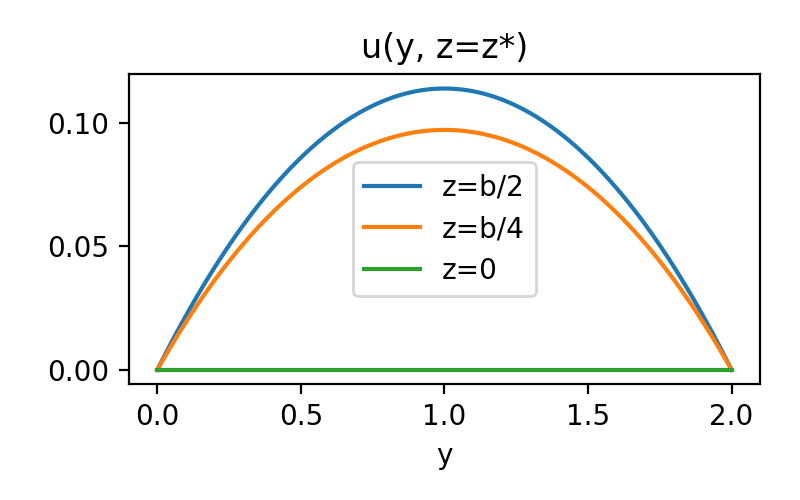
\includegraphics[scale=1]{u(y)}
\centering
\caption{u(y)}
\label{fig:u(y)}
\end{figure}

\begin{figure}[H]
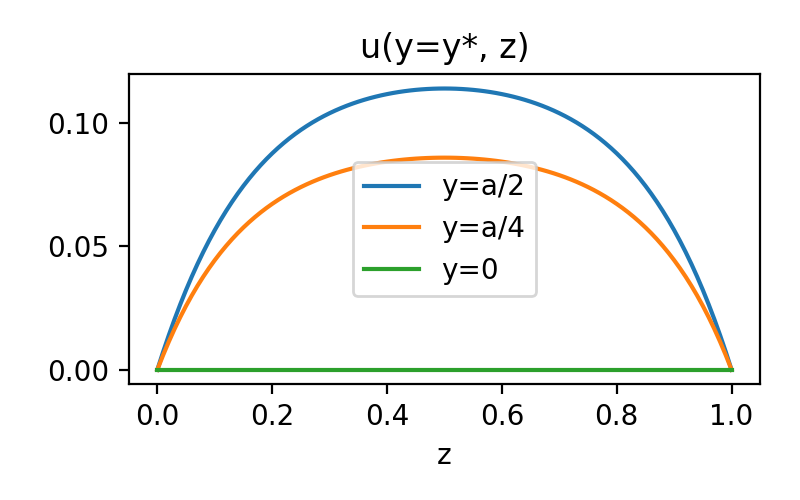
\includegraphics[scale=1]{u(z)}
\centering
\caption{u(z)}
\label{fig:u(z)}
\end{figure}

\end{solution} 

\begin{solution} 

\begin{figure}[H]
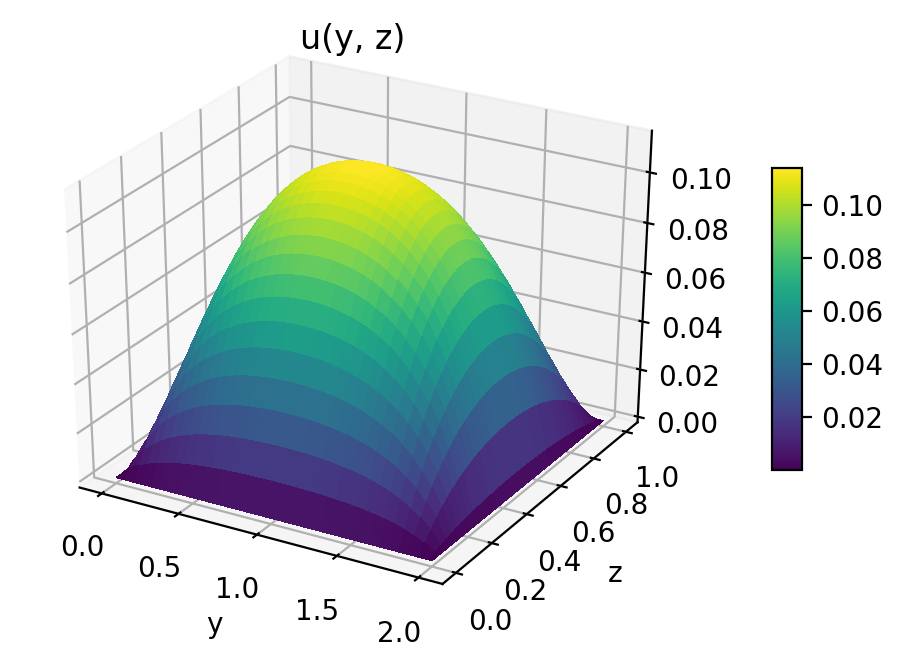
\includegraphics[scale=1]{surface_plot}
\centering
\caption{Surface plot of u(y, z)}
\label{fig:surf}
\end{figure}

See HW1P2\_plot.ipynb for the code generating the plots.

\end{solution} 

\newpage
  \section{Problem 3: The Finite Element Method}

  Consider the steady one-dimensional advection-diffusion-reaction equation,
  \begin{align}
    a\partial_{x}u -\lambda u - k\partial_{x}^{2}u = f, \qquad x\in\left(0, 1\right)
    \label{eq:adv-diff-rxn}
  \end{align}
  with boundary conditions 
  \begin{align}
    u\left(0\right) = u_{0}, \quad -k\partial_{x}u\left(1\right) = b_{1}.
    \label{eq:adr_bcs}
  \end{align}
  In~\eqref{eq:adv-diff-rxn}, $a$ is the constant advection speed, $\lambda > 0$ is the constant reaction coefficient, and $k>0$ 
  is the constant diffusion coefficient.  

    \subsection{Weak Form}
    Write the weak form corresponding to the strong form~\eqref{eq:adv-diff-rxn}.  Be sure to specify all function spaces. Don't forget to include any boundary terms.\\

    \begin{solution}
Let $w$ be a test function which we will multiply times the stronghold function, and integrate over the domain, where $w(0) = 0$.

\begin{align}
\int_0^{1} w(a \partial_x u - \lambda u - k \partial_x^2 u)dx &= \int_0^1 fwdx\\
\int_0^{1} w a \partial_x u dx- \int_0^{1} w \lambda u dx - \int_0^{1} kw\partial_x^2 u dx &= \int_0^1 fw dx\\
\int_0^{1} w a \partial_x u dx- \int_0^{1} w \lambda u dx -wk\partial_x u \Big |_{0}^1 + \int_0^1 k \partial_x w \partial_x u dx &= \int_0^1 fw dx\\
\int_0^{1} w a \partial_x u dx- \int_0^{1} w \lambda u dx - (k w(1)\partial_x u(1)) + \int_0^1 k \partial_x w \partial_x u dx &= \int_0^1 fw dx\\
a \int_0^{1} w \partial_x u dx - \lambda\int_0^{1} w u dx + k\int_0^1 \partial_x w \partial_x u dx &= \int_0^1 fw dx + b_1 w(1)
\end{align}

Let the following function spaces be defined as follows:\\

$S = \left\{ u | u \in H^{(1)}, u(0) = u_0 \right\}$ and $V = \left\{ v | v \in H^{(1)}, v(0) = 0 \right\}$ \\

Additionally, let $u^h \in S^h \subset S$, $w^h \in V^h \subset V$, and $u^h \in V^h$. We can now proceed to write the Galerkin statement below.

\end{solution}

    \subsection{Galerkin Statement}
    From the weak form, write the Galerkin statement.  Again, specify all function spaces.\\
    
    \begin{solution}
Find $u^h \in V^h$ such that $\forall$ $w^h \in V^h$:\\

$a \int_0^{1} w^h \partial_x u^h dx - \lambda\int_0^{1} w^h u^h dx + k\int_0^1 \partial_x w^h \partial_x u^h dx = \int_0^1 fw^h dx + b_1 w^h(1)$\\

Now, let us assume that $u^h$ has the following $u^h = v^h + g^h$ where $g^h(0) = u_0$, still meeting the conditions to be in the $V^h$ function subspace. We proceed to rewrite the function in the following form:\\

$$a \int_0^{1} w^h (\partial_x v^h + \partial_x g^h) dx - \lambda\int_0^{1} w^h (v^h + g^h) dx + k\int_0^1 \partial_x w^h (\partial_x v^h + \partial_x g^h) dx = \int_0^1 fw^h dx + b_1 w^h(1)$$

\begin{dmath}
a \int_0^{1} w^h \partial_x v^h dx - \lambda\int_0^{1} w^h v^h dx + k\int_0^1 \partial_x w^h \partial_x v^h dx= \int_0^1 fw^h dx + b_1 w^h(1) - a \int_0^{1} w^h \partial_x g^h dx + \lambda\int_0^{1} w^h g^h dx - k\int_0^1 \partial_x w^h \partial_x g^h dx
\end{dmath}
\end{solution}

    \subsection{Finite Element Discretization} Introduce the finite element basis and arrive at a linear algebra problem.  Clearly define the form of all resulting matrices.  You may write everything in terms of the basis functions (i.e. there is no need to directly compute the entries of the matrices).\\

    \begin{solution}
Now, let 

$$w^h = \sum_{A=1}^{n}W_A N_A(x) \qquad N_A(1) = 0, \, \forall \, A=[1, ..., n]$$
$$u^h = \sum_{B=1}^{n}U_B N_B(x) + u_0 N_{n + 1}(x) \qquad N_B(0) = 0 , \, \forall \, B=[1, ..., n], \, N_{n+1}(0) = 0$$\\

Therefore, defining: 

$$v^h = \sum_{B=1}^{n}U_B N_B(x)$$

$$g^h = u_0 N_{n + 1}(x) $$

We proceed now to plug these values into the Galerkin Statement:

\begin{dmath}
a \int_0^{1} \Big(\sum_{A=1}^{n}W_A N_A(x)\Big) \partial_x \Big(\sum_{B=1}^{n}U_B N_B(x)\Big) dx - \lambda\int_0^{1} \Big(\sum_{A=1}^{n}W_A N_A(x)\Big) \Big(\sum_{B=1}^{n}U_B N_B(x)\Big) dx + k\int_0^1 \partial_x \Big(\sum_{A=1}^{n}W_A N_A(x)\Big) \partial_x \Big(\sum_{B=1}^{n}U_B N_B(x)\Big) dx= \int_0^1 f \Big(\sum_{A=1}^{n}W_A N_A(x)\Big) dx + b_1 \Big(\sum_{A=1}^{n}W_A N_A(1)\Big) - a \int_0^{1} \Big(\sum_{A=1}^{n}W_A N_A(x)\Big) \partial_x \Big(u_0 N_{n + 1}(x)\Big) dx + \lambda\int_0^{1} \Big(\sum_{A=1}^{n}W_A N_A(x)\Big) \Big(u_0 N_{n + 1}(x)\Big) dx - k\int_0^1 \partial_x \Big(\sum_{A=1}^{n}W_A N_A(x)\Big) \partial_x \Big(u_0 N_{n + 1}(x)\Big) dx
\end{dmath}

\begin{dmath}
\sum_{A=1}^{n}W_A \Bigg[ a \int_0^{1} N_A(x) \partial_x \Big(\sum_{B=1}^{n}U_B N_B(x)\Big) dx - \lambda\int_0^{1} N_A(x) \Big(\sum_{B=1}^{n}U_B N_B(x)\Big) dx + k\int_0^1 \partial_x N_A(x) \partial_x \Big(\sum_{B=1}^{n}U_B N_B(x)\Big) dx - \int_0^1 f N_A(x) dx - b_1 N_A(1) + a \int_0^{1} N_A(x) \partial_x \Big(u_0 N_{n + 1}(x)\Big) dx - \lambda\int_0^{1} N_A(x) \Big(u_0 N_{n + 1}(x)\Big) dx + k\int_0^1 \partial_x N_A(x) \partial_x \Big(u_0 N_{n + 1}(x)\Big) dx \Bigg] = 0
\end{dmath}
\end{solution}
\begin{solution}
\begin{dmath}
\sum_{A=1}^{n}W_A \Bigg[ \sum_{B=1}^{n}U_B \Bigg( a \int_0^{1} N_A(x) \partial_x N_B(x) dx - \lambda\int_0^{1} N_A(x) N_B(x) dx + k\int_0^1 \partial_x N_A(x) \partial_x N_B(x) dx \Bigg) - \int_0^1 f N_A(x) dx - b_1 N_A(1) + a \int_0^{1} N_A(x) \partial_x \Big(u_0 N_{n + 1}(x)\Big) dx - \lambda\int_0^{1} N_A(x) u_0 N_{n + 1}(x) dx + k\int_0^1 \partial_x N_A(x) \partial_x \Big(u_0 N_{n + 1}(x)\Big) dx \Bigg] = 0
\end{dmath}

To simplify the formula, let us redefine some of the expressions above:

\begin{align}
\kappa_{AB} &= a \int_0^{1} N_A(x) \partial_x N_B(x) dx - \lambda\int_0^{1} N_A(x) N_B(x) dx + k\int_0^1 \partial_x N_A(x) \partial_x N_B(x) dx \\
F_a &= \int_0^1 f N_A(x) dx\\
G_a &= a \int_0^{1} N_A(x) \partial_x \Big(u_0 N_{n + 1}(x)\Big) dx\\
H_a &= b_1 N_A(1)\\
I_a &= \lambda\int_0^{1} N_A(x) u_0 N_{n + 1}(x) dx\\
J_a &= k\int_0^1 \partial_x N_A(x) \partial_x \Big(u_0 N_{n + 1}(x)\Big) dx\\
\mathbf{F}_A &= F_a + G_a - H_a + I_a - J_a
\end{align}

Therefore, rewriting our expression above as:

\begin{dmath}
\sum_{A=1}^{n}W_A \Big[ \Big( \sum_{B=1}^{n}U_B( \kappa_{AB}) - \mathbf{F}_A\Big] = 0
\end{dmath}

In order for the expression to hold, the following must be true:\\

$$\sum_{B=1}^{n}U_B( \kappa_{AB}) = \mathbf{F}_A$$
\end{solution}

\newpage
  \section{Problem 4: Implementation}
  We wish to use the finite element method to solve 
  \begin{align}
    - \partial_{x}^{2} u = f\lr{x}, \qquad x \in \lr{0, 1} \\
    -\partial_{x}u\lr{0} = \mathcal{h}, \quad u\lr{1} = \mathcal{g}
  \end{align}
  for $u\lr{x}$ where $f\lr{x}$ is a known forcing function and $\mathcal{g}$ and $\mathcal{h}$ are constant boundary data.

  Write a one-dimensional finite element code that uses piecewise linear finite elements to solve for $u\lr{x}$.  The
following specifications are required:
  \begin{itemize}
    \item The code should work for any constant $\mathcal{g}$ and $\mathcal{h}$ as well as arbitrary $f\lr{x}$.  These will be inputs to the
code.
    \item Other inputs should include the domain size.  You have some flexibility on how to do this.  For example, you may
pass in a fully-formed mesh if you wish.  Alternatively, you can require the user to specify the number of elements from
which your code can compute the uniform mesh size.
      \begin{itemize}
        \item \textbf{Note:} You may assume a uniform mesh.
      \end{itemize}
    \item The code \textbf{must} use the local point of view.  That is, loop over individual elements and perform the finite
element assembly operation to form the global stiffness matrix and force vector.
    \item Use Gaussian quadrature to perform the integrals.  Although not strictly necessary here, it will give you some
intuition for how things are actually done.
    \item You may use an external library to solve the resulting linear system.
    \item Use must use a compiled language such as \texttt{C}, \texttt{C++}, or (modern) Fortran.
    \item Try to submit your job on Odyssey!
  \end{itemize}

  Some other things you may want to consider are the following:
  \begin{itemize}
    \item Start simple.  A natural progression may be the following:
      \begin{itemize}
        \item Select $f = 0$, $g = 0$ and $h = 1$ to begin.  The exact solution will be $u = 1 - x$.
        \item Then make $g = 1$, $h = 1$, $f = 0$.  The exact solution will be $u = 2 - x$.
        \item Finally, try $g = 1$, $h = 1$, and $f = 1$.  The exact solution will be $u = 2 - x + \dfrac{1}{2}\lr{1 -
x^{2}}$.
        \item At this point, you will have some confidence in your code.  This is called code verification.  You can try more
complicated $f\lr{x}$ if you'd like to.
      \end{itemize}
    \item Organize your code into separate files.  Use a \texttt{Makefile} to do the linking.
      \begin{itemize}
        \item You may want to have files for the following:
          \begin{itemize}
            \item Quadrature routines 
            \item Stiffness matrix routines 
            \item Right-hand-size (RHS) routines
          \end{itemize}
        \item Feel free to consider other code designs.
      \end{itemize}
  \end{itemize}
  
   \begin{solution}
Using the C programming language, we constructed the following finite element method implementation:

\begin{itemize}
\item[] \textbf{main.c} : allows the user to specify his/her values for the function $f$, and boundary conditions for $g$ and $h$.
\item[] \textbf{construct\_matrix.c} : computes $\kappa _{AB}$
\item[] \textbf{gaussian\_quadrature.c} : uses gaussian quadrature to estimate integration values for various functions specified within the file
\item[] \textbf{tridiag\_solver.c} : uses the $lapacke$ library to solve a linear system described by Ax = y for x. 
\end{itemize}

To specify the values for $f$, $g$, and $h$, there is a section in the main function in \textbf{main.c} file, under the section for \texttt{Variable initialization}.

To verify that our solution made sense we graphed our output in a Jupyter notebook that can be found in the same directory as the rest of our code.\\

For $f = 0$, $g = 0$ and $h = 1$, the exact solution will be $u = 1 - x$.

\begin{center}
    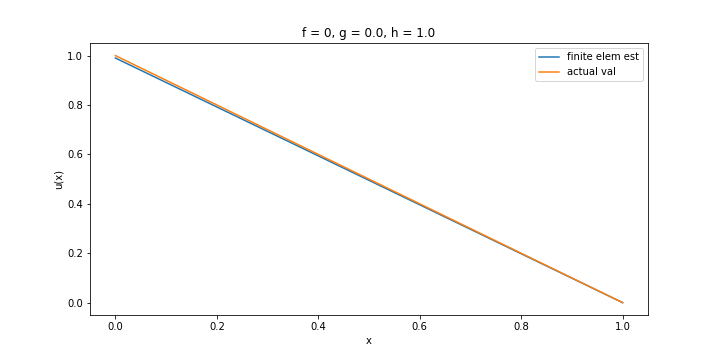
\includegraphics[scale=0.5]{DavidPineiro/f0_g0_h1.png}
\end{center}


\end{solution}
\begin{solution}
For $g = 1$, $h = 1$, $f = 0$, the exact solution will be $u = 2 - x$.

\begin{center}
    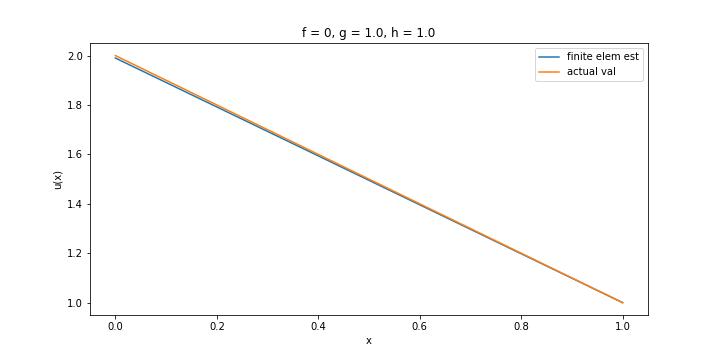
\includegraphics[scale=0.5]{DavidPineiro/f0_g1_h1.png}
\end{center}

For $g = 1$, $h = 1$, and $f = 1$, the exact solution will be $u = 2 - x + \dfrac{1}{2}(\lr{1 - x^{2}})$.

\begin{center}
    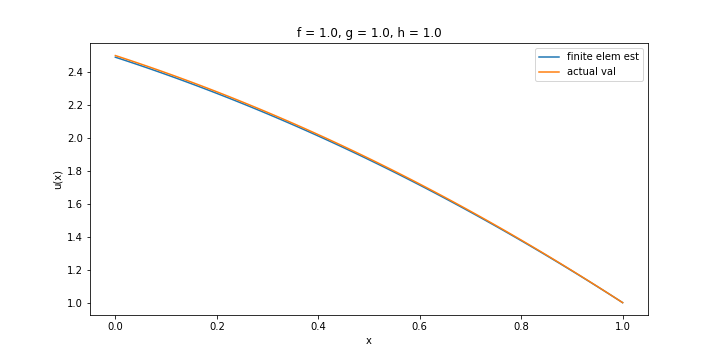
\includegraphics[scale=0.5]{DavidPineiro/f1_g1_h1.png}
\end{center}

Therefore, we verified our solution and have confidence in our code.

\end{solution}

\end{document}
